\documentclass[11pt]{article}
\usepackage{threeparttable}
\usepackage{rotating}
\usepackage{xcolor}
\usepackage{subfig}


%_ PACKAGES __________________________________________________________________________ %
	
    %__ INPUT/OUTPUT LANGUAGE _________________________________ %
    \usepackage[USenglish]{babel}
    \usepackage[utf8]{inputenc}
    \usepackage[T1]{fontenc}
    %\usepackage{indentfirst}

    %__ MATH __________________________________________________ %
    \usepackage{amsfonts}
    \usepackage{amssymb}
    \usepackage{amsmath}
    \usepackage{amsthm}
    \usepackage{bbm}
    
    %__ THEORY __________________________________________________ %
    \newtheorem{name}{Printed output}
	\newtheorem{lemma}{Lemma}
	\newtheorem{prop}{Proposition}
	\newtheorem{cor}{Corollary}
	\theoremstyle{definition}
	\newtheorem{definition}{Definition}

    %__ GRAPHS & TABLES________________________________________ %
    \usepackage{graphicx}
    \usepackage{subfig}
    \usepackage{booktabs}
    %\usepackage{multirow}
    \usepackage{array}
    \usepackage{caption}
    %\usepackage{subcaption}
    %\usepackage[flushleft,online,para]{threeparttable}
    
    %\usepackage{parskip}                       % WHAT IS THIS FOR?

    \usepackage{floatrow}
        \floatsetup[table]{style=plaintop}     % LEAVE TABLE CAPTIONS AT THE TOP
    %\usepackage[nolists,nomarkers]{endfloat}             % PUT FIGURES AT THE END OF DOCUMENT; DOESN'T WORK WITH \usepackage{float}

    \usepackage{tabularx}
        \newcolumntype{Z}{>{\centering\arraybackslash}X}
        \newcolumntype{L}{>{\raggedright\arraybackslash}X}

    \usepackage{dcolumn}
        \newcolumntype{d}[1]{D{.}{.}{#1}}

    \usepackage{rotating}                      % for **sideways**tables
    \usepackage{lscape}
    \usepackage{pdflscape}

    %__ BIBLIOGRAPHY __________________________________________ %
    \usepackage[round]{natbib}

    %__ PDF, DISPLAY & PRODUCTIVITY ___________________________ %
    \usepackage{xcolor}
        \definecolor{darkblue}{rgb}{0,0,0.4}
    \usepackage{hyperref}
        \hypersetup{
            colorlinks = true,
            linkcolor = darkblue,
            citecolor = darkblue,
            pdfborder = 0 0 0,
            pdfdisplaydoctitle = true,
            pdfhighlight = /N,
            pdfpagelayout = OneColumn,
            pdfpagemode = UseNone,
            pdfstartview = {FitH},
            pdfauthor = {{AB, CF \& JR}},
            pdftitle = {{DYN}},
            pdfsubject = {{}}
        }

    \usepackage[textsize=footnotesize, colorinlistoftodos, textwidth=4cm, obeyDraft]{todonotes}
    %\usepackage{fixme}
        % commands \fxnote; \fxwarnin; \fxerror; \fxfatal
        % \fxsomething{options}{note}{TEXT}* highlights the TEXT

    \usepackage{geometry}
        \geometry{verbose,tmargin=2.5cm,bmargin=2.5cm,lmargin=2.5cm,rmargin=2.5cm}
    \usepackage{setspace}
        \onehalfspacing

    \usepackage[bottom, multiple]{footmisc}    % keep footnotes at the bottom of the page, and allow for multiple footnotes at one place.

    \usepackage{verbatim}
    \usepackage[normalem]{ulem}     % strikethrough fonts
    \usepackage{mathpazo}

    %\usepackage{syntonly}       % if uncommented, this will prevent latex to produce
    %    \syntaxonly             %   any output. latex will only check for syntax.
    %\usepackage[displaymath,tightpage]{preview}
    %\graphicspath{{//graphs/}}

    %__ APPENDIX _____________________________________________ %
    \usepackage[toc,page]{appendix}

%__ COMMANDS _________________________________________________________________________ %
    \newcommand{\mc}{\multicolumn}
    \newcommand{\lbar}{\underline}
    \newcommand{\ubar}{\overline}




\title{\textbf{Can Monitoring and Transparency Make Food Safer, and at What Cost?}}

\author{Jason Huang}

\date{\bigskip \today}

% _ DOCUMENT _________________________________________________________________________ %

\begin{document}

\newcommand{\cfbox}[2]{%
    \colorlet{currentcolor}{.}%
    {\color{#1}%
    \fbox{\color{currentcolor}#2}}%
}

\maketitle

\begin{abstract}

I estimate the impact of food inspections on restaurant cleanliness by estimating how inspection results affect subsequent inspection results and 311 complaint calls. To deal with the endogeneity of the inspection results, I exploit the random assignments of inspectors and construct inspector-specific measures of stringency as an instrumental variable. I find that this variable is highly predictive of not only the total scores but also the specific violations that are cited, despite the random assignment process that results in similar restaurant characteristics across inspectors. I find that, on the margin, more citations leads to better subsequent inspections. I also find that the establishments not only address the areas for which they received citations but also improve in other areas, suggesting complementarity across multiple dimensions of cleanliness. Furthermore, I find that consumers also respond to these improved sanitation conditions by finding lower probabilities of receiving 311 complaint calls inspection results that do not contribute to public information have little effect on call frequencies. But inspection results that contribute to lower letter grades lead to a significant increase in calls. Taken together, my findings suggest that the violation citations have incentivize restaurants to improve, but these efforts are not noticed by customers. Instead, consumers react mostly to the letter grades, which may at times not fully reflect the underlying qualities. Current findings suggest that showing a numerical score instead of or concurrently with the letter grades can be more informative. This paper also has important implications for other cities as they plan to design or modify their methods of displaying their food inspection results.

\textit{JEL: D02, D81, D82, K32, L51}\\
\end{abstract}
\thispagestyle{empty} \newpage

\onehalfspacing \setcounter{page}{1}

\section{Introduction}

Food hygiene at restaurants is a great public health concern. The CDC estimates that over 3 million incidents of food-borne illness occur in the US annually, with 60\% of the cases resulting from  dining in restaurants\footnote{Surveillance for Food borne Disease Outbreaks United States: 2013 Annual Report. Available: https://www.cdc.gov/foodsafety/pdfs/foodborne-disease-outbreaks-annual-report-2013-508c.pdf}. Unlike food quality or service, which consumers can easily observe, food sanitation remains opaque to consumers since most diners cannot venture back to the kitchens and monitor the food preparation process. Local health departments have long conducted regular food inspections to ensure that restaurants meet certain hygiene standards. In the last two decades, however, major cities have started make these inspection results publicly available. In the case of New York City (NYC), starting from July 2010, the Department of Health and Mental Hygiene (DOHMH) has required restaurants to post letter grades on their entrance windows. During each inspection, the inspector calculates a score based on the number of violations and their severities. The numerical score is then converted to a letter grade. 

This paper estimates the causal impact of NYC's food inspection results on restaurant compliances and customer perceptions, measured by frequencies of 311 complaints calls. Inspection results can potentially influence restaurant behaviors through for two reasons. First one is monetary. The scores determine the letter grades restaurants post on their entrance windows. These grades can influence consumer demand and affect revenues. The second one is behavior. restaurants may improve by learning from previous mistakes through the citations. Restaurants may commit violations not because they are profit maximizing and purposefully cutting enough corners to equate the marginal savings with the expected marginal cost of penalties from DOHMH. Instead, restaurants may be simply making mistakes because of lack of knowledge or experience.\footnote{A potential reason is that scores are directly associated with monetary penalties. Each violation is associated with a fine, and the amount of fine depends on the severity cited by the inspector. However, the amounts of these fines are very small, ranging from 200 to 1000 per violation.} Given that cleanliness is a multi-dimensional task, I examine how the distribution of citations impact the distributions of efforts across these dimensions. Finally, I test whether consumers behaviors respond to changes in restaurant hygiene efforts by measuring the changes in the frequencies of 311 complaint calls. The inspection results may affect consumer behaviors through two channels. In the first channel, worse results incentivize restaurants to make substantive improvements, which lead to decreases in calls. In the second channel, worse results lead to lower grades, causing consumers to view the establishment more negatively and more likely to complain. 

The initial results find that, on the margin, restaurants respond to poor inspection results by improving their cleanliness, as measured by improved scores from subsequent inspections. Furthermore, I find that the establishments improve by not only focusing on the areas for which they received citations but on almost every aspect. In regards to the complaint calls, I find that inspection results that do not contribute to letter grades have minimal effect. However, for inspection results that contribute to the posted letter grade, failing to earn the top grade leads to more than 200\% increase in the number of complain calls relative to the average of . The results suggest that the cleanliness of restaurants improve in response to citations, but along dimensions that are not easily visible to consumers. Instead, consumers react mostly to the letter grades, which may at times not fully reflect the underlying sanitation qualities. A simple model to explain this result is that a customer calls to complain whenever one's perceived experience at a restaurant drops below a certain threshold. Ceteris paribus, a lower letter worsens the perceived experience, making the complaint call more likely. 

An empirical challenge to studying the impact inspection is that the variable of interest, the inspection results, is endogenous. It includes both the effects of monitoring and compliance. For example, suppose we find that restaurants that had high numbers of citations tend to have high number of citations in the future. Do more citations lead to worse compliance or do restaurants that did poorly in the past continue to do poorly in future? This paper uses the random assignment of food inspectors to inspections for restaurants in New York City as an instrumental variable to overcome the endogeneity of inspection results. As different inspectors have different levels of stringencies, the results that restaurants receive are partly determined by chance.\footnote{Other areas of research that have used this random assignments of decision makers to recover causal impacts of include the impact of incarceration on recidivism \citep{bhuller_16}, the effect of disability insurance on labor supply \citep{Maestas_13}, and the impact of foster care system on child outcomes \citep{Doyle_07}.}

A growing literature has focused on the role of transparency to improve food sanitation and reduce food-borne illness. The first type is certification, or what \cite{Ho_2012} calls targeted transparency. Letter grade system, first introduced in Los Angeles and later adopted by New York City is one example of certification. \cite{jie_leslie_05} and \cite{Simon_05} study the introduction of the grading system in Los Angeles in 1998 and find strong evidence for a decrease in hospitalization for foodborne illnesses in jurisdictions after the enactments of the grading systems. \cite{jie_leslie_05} argue that the reduction is driven by people cooking more at home and eating out less. \cite{Wong_at_el_2015} and \cite{Meltzer_2015} study New York City's food inspection program. They use inspection scores to measure restaurant cleanliness. After finding that improved sanitation scores and lower violation fines followed the reform, they conclude that the reform improved sanitation practices. These papers looks at impact of the overall inspection program while I study the effect of individual inspections. \cite{Filion_Powell_09} document the growing popularities of these grading programs across the globe. The second type of transparency arise from customer reviews. \cite{Luca_13} use Yelp reviews to predict health code violations, and they argue that inspection selection can be optimized based on information from social media. However, sending food inspectors to restaurants for inspections remains as the most direct tool of enforcement, and understanding the impact of these inspections on compliance remains important. Hence, I see this study about monitoring and detection as a complement to instead of a substitute of studies about the role of transparency. 

This paper also relates to a broad literature that studies the connection between government monitoring and compliance. Researchers have explored this issue in other areas such as taxation (\cite{Feinstein_91}, \cite{Kleven_etal_10}, \cite{Gemmell_Ratto_12}), workplace safety \citep{levine_etal_12}, nuclear power plants \citep{Feinstein_89}, and environmental protection \citep{Duflo_Greenstone_14}. \cite{Jin_Lee_12} and \cite{Jin_Lee_14} also look at the interaction between food inspectors and restaurants. But they focus on the inspectors' behaviors and detection technology, while this paper asks a related but different question of how restaurants respond to these inspections results. 

The rest of the paper proceed as follows. Section \ref{background} discusses the New York City's food inspection program. Section \ref{data} describes the food inspection and 311 data. Section \ref{IV} discusses the construction of the instrumental variable and describes various validity tests. Section \ref{empirical_sec} presents the main empirical strategy and shows the results. Section \ref{conclude} ends this draft with a discussion of the policy implications and the steps going forward. 

\section{New York City Food Inspection and Grading System}
\label{background}

New York City's DOHMH oversees the food safety program. It sends out food inspectors to restaurants to conduct inspections. Each restaurant receives at least one inspection a year. Starting in 2005, the city implemented a numerical scoring system. It outlined ninety-eight violations, broken into eight categories: food temperature, food source (general and critical), food protection, facility design, personal hygiene, vermin/garbage, and facility maintenance. Each violation is associated with a range of scores, and the inspector assigns the numerical value that reflects the severity of the violation. For example, a violation 10F for not non-food contact surface improperly constructed is worth from 2 to 5 points, depending on how many of these surfaces the inspector finds\footnote{See Food Service Establishment Inspection Procedures Handbook: 

http://www1.nyc.gov/assets/doh/downloads/pdf/about/healthcode/health-code-chapter23.pdf. }.  

Starting in 2010, the sum of the scores were converted to letter grades, A, B, C, based on the following cutoffs. Score between 0 to 13 earns an A, between 14 to 27 earns a B, and 28 or above earns a C. In addition, the city required the restaurants to post these letter grades on the entrance so that they are clearly visible to the customers. The grading policy also changed the inspection cycles. It introduced dual inspection cycles, which involved the a random initial inspection and a possible re-inspection within a month if the initial inspection results in a letter grade lower than an A. During the time in between the initial inspection and re-inspection, restaurants can either post their assigned letter grade or a sign saying "Grade Pending." The score from re-inspection is then used to determine the letter grade the restaurant posts until the next initial inspection, and the previous initial inspection result has no effect. Inspectors to both cycles are randomly assigned so rarely do the same inspector inspect a restaurant twice in a row. Finally, the time between an initial inspection and the subsequent initial inspection depends on the inspection results from the original inspection. If the initial inspection score is lower than 14, the subsequent inspection occurs in roughly a year. If the score is between 14 and 27, the median time until the next inspection is 201 days. If the score is greater than 27, the median length until the next inspection is 176 days. 

DOHMH may temporarily close a restaurant for two reasons. The first reason is that the establishment poses a public health hazard that cannot be addressed by the end of the inspections. Such hazard includes issues such hot food not cooked to high enough temperature or cold food not stored at low enough temperature, presence of unpasteurized milk, or harmful noxious gas detected. The second reason is that restaurants receive scores above 28 for three consecutive inspections. If closed, DOHMH immediately posts a closure sign on the window. To reopen, the establishment must submit a written statement to DOHMH that describes the steps it has taken to correct the violations. Then re-opening inspection occurs. The median time between closure and re-opening inspection is 4 days, with 95\% of the cases occurring within 24 days. The establishment can re-open if it passes the re-opening inspection, but it receives its next initial inspection within three months. Repeat violations may prompt DOHMH to shutdown an establishment for longer or permanently. 

All inspections are conducted with a handheld computers in which the inspectors record the violations. The sum of the individual scores exceeding certain threshold triggers either re-inspections or closure of the restaurant. The average inspection takes one hour and forty-five minutes.  

\section{Data}
\label{data}
\subsection{Food Inspection Data}

The main data source is the universe of food inspection results conducted by New York City's Department of Health and Mental Hygiene (DOHMH) from July 2007 to September of 2016. Each observation in the data corresponds to a violation cited during each inspection. It has information on the date of the inspection, the type of inspection (whether initial inspection or re-inspection), anonymized ID of the inspector, the total score from all the violations, date of adjudication if it occurred, and the modified score after adjudication. It also has the name, street address, zipcode, cuisine type, service type, and venue type of the establishment. 

This study focuses mainly on the inspections conducted after the enactment of the grading system, which occurred on July 2010. While sources say the implementation was swift, I use all inspections that occurred after October 1st of 2010 to give 3 month buffer to account potential lags.\footnote{\cite{Ho_2012} says that the actual law was enforced on July 15, 2010.} In the period following the grading system, on which this paper focuses, I see over 337,000 inspections, which include both initial inspections and re-inspections, across over 44,000 establishments. Figure \ref{pipeline} shows the distributions of inspection types across the inspection types. We see that over 60\% of initial inspections earn scores higher than 13, resulting in re-inspections. Of the re-inspections, 14.2\% earn Cs, 37.7\% earn Bs, and the remaining earn As. But almost 90\% of re-inspections that do not earn As go to adjudication, with a bit over half getting modified scores that result in improved grades and over 80\% resulting in lower modified scores. 

Table \ref{sum_stat} presents summary statistics for both the restaurant samples and inspection samples. By comparing the two samples, we can see whether inspections tend to skew towards certain types of restaurants. The statistics appear fairly comparable across the two samples, with restaurants that have counter service being inspected more often and those with takeout service inspected less often. 
\subsection{311 Calls}

New York's 311 is a special telephone number designated for non-emergency requests to municipal services. The phone line also served as a way to report complaints, such as sighting of rodents or food poisining, against retail food establishments to DOHMH. The data contain the date of the call, the types of complaints, and the address of the incident. 

The 311 calls are matched to the food inspection data based on the address using fuzzy string matching. The appendix provide more detail on the matching process. 

\subsection{Descriptive Analysis: Bunching Around Thresholds}

As documented in other economic literatures, the discontinuous mapping from integral scores to discrete letter grades creates jumps in incentives and leads to bunching in the score distributions\footnote{See \cite{Gourio_Roys_14} for discontinuity of firm sizes caused by size-based regulations.}. More specifically, as shown in the left plot of figure \ref{bunching}, the distribution of scores from initial inspections clearly show bunching around the cutoff between an A and a B at 13. We do not see any bunching above 13 since all those inspections re-inspections follow and those scores do not contribute to the final  and those restaurants often opt to post Grade Pending in the meantime. In the right plot in figure \ref{bunching}, we see bunching around both 13 and 27 in the scores from re-inspections since those scores contribute to the determination of the letter grades. 

Strategic behaviors of both the inspectors and the restaurants can contribute to the observed bunching in the score distribution. Some potential reasons for inspectors to bunch during the first inspection include saving extra trips for re-inspections or the administrative costs of adjudications. But given that the same inspector does not inspect conduct the re-inspection, and the adjudication is handled by another department, this explanation is unlikely. The bunching may be driven by restaurant behaviors. The inspection worksheet is publicly available, so the restaurants may that are around the threshold between grades may exert extra effort to improve. A final reason, which is a behavioral explanation, may be that inspectors experience awkwardness handing out a score that is a point or two what is needed to earn a better grade. 

\section{Stringencies of Inspectors as Instrumental Variable}
\label{IV}
According to staff of DOHMH, whenever a restaurant needs to be inspected, whether for an initial inspection or a re-inspection, a inspector is randomly assigned to inspect that establishment. Inspectors do not specialize in any particular geographies or types of restaurants, so every restaurant at any point in time should be equally likely to receive any of the inspectors. In the next subsections, I discuss how I construct the instrumental variable and show its predictive power on the endegenous variable. 
 
\subsubsection{Inclusion Restriction}
\label{IV_construct}
The inclusion restriction of a instrumental variable requires it to have high predictive power on the endogenous variable. In this case, we need our inspector stringency to be highly statistically correlated with the scores that the inspector assigns to the restaurants. I calculate the instrumental variable for each inspection by computing the average score that the assigned inspector gives to all the other restaurants that the inspector has inspected for that inspection type (initial or re-inspection). Specifically, I define the instrument between restaurant $i$ and inspector $j$ of inspection type $p$ as
\begin{align*}
    Z_{ijp} = \frac{1}{n_{jp} - I_{ijp}} \left( \sum_{kjtp\neq ijtp}  SCORE_{kjtp}\right)
\end{align*}
where $n_{jp}$ is the total number of type $p$ inspections conducted by inspector $j$, $I_{ijp}$ is the total number of type $p$ inspections inspector $j$ has conducted at restaurant $i$, and $SCORE_{kjtp}$ is the score inspector $j$ gave to restaurant $k$ on date $t$ for an inspection type $p$.\footnote{The types of inspections can be either initial inspection or re-inspection. } 

Figure \ref{first_stage_fig} plots the distribution of the inspector average scores. The histogram shows a considerable amount of heterogeneity in terms of inspectors' levels of stringencies\footnote{See \cite{Feinstein_89}, \cite{Feinstein_91}, and \cite{Macher_11} for additional documentation of inspector heterogeneity pertaining to IRS examiners, nuclear power plant inspectors, FDA regulators, respectively.}. Figure \ref{first_stage_fig} also shows the fitted value of locally weighted regression of the inspection scores on the inspectors' leave-out average scores\footnote{I use a bandwidth of 0.5.}. The inspection scores and the inspector average scores follow a monotonic relationship, closely tracing along the 45$^\circ$ line. The plot suggests that being inspected by a more stringent inspector leads to a higher score. 

We set up the first stage of our two-stage least square analysis here. 
\begin{align}
score_{it} = \gamma Z_{it} + \delta_i + \tau_t + \epsilon_{it}
\label{first_stage_eq}
\end{align}
Table \ref{first_stage_reg} shows the first stage result of \eqref{first_stage_eq}. I show the results of both with and without restaurant fixed effects. We see that the point estimates are around 1, which suggests that an inspection done by an inspector with a 1 point higher average score increases the expected inspection score by 1 point. The estimates are also highly statistically significant, suggesting that the inspector stringency is not a weak instrument. 

\subsection{Assessing the Randomness of Inspector Assignment}

While we cannot directly test for the randomness of the inspectors' assignment process, we can test for some empirical patterns that random assignment implies.  

The first implication of random assignment is that the inspector propensity should not be correlated with observables of restaurants to which one is assigned. Hence, we test whether restaurant observable characteristics have predictive power of the stringency levels of the inspectors assigned to them. If the assignments are random, the covariates should all be small and statistically insignificant. For example, a coffee shop in Brooklyn should have the same chance of getting a strict inspector than a Michelin five star restaurant in Manhattan. Table \ref{cond_ind} shows the regression results of inspection scores and inspector leave-out average score on various restaurant characteristics and lag terms. We see that all the covariates are highly statistically significant for the score regression. In the second column, which the depend variable is the inspector propensity but includes inspections conducted by inspectors who have at least 50 inspections, most of the covariates have no statistical significance and the point estimates are very small. There are few covariates, such as Pizza/Italian cuisine, or whether the establishment offers buffet or cafeteria service, that are statistically significant at 90\% or higher level. However, their point estimates are fractions of those in the score regression. Calculating inspector propensity using only 50 inspections may cause some covariates to be significant by chance. The third column restrict the sample to inspections done by inspectors with at least 650 inspections. We see that the covariates that were significant in the second columns are no longer significant. 

A second implication of the randomness is that the inspections each inspector conduct should not be geographically clustered, and each geographic area should not be inspected by only a few inspectors. To test this claim, I calculate the Herfindahl-Hirschman index (HHI) of the zipcodes of the restaurants each inspector has inspected and the HHI of the inspectors that have inspected each zipcode. The results are presented in figure \ref{zip_herf}. The red dotted lines represent the HHI of zipcodes and inspectors under the perfect random case\footnote{Because inspections are not uniformly distributed, the baseline is calculated based on the sample distributions of inspectors across zipcodes}. The takeaway from the figure is that, while no zipcode or inspector exhibit a perfectly random distribution, I find no evidence that inspectors tend to focus on a small geographic area or that certain zipcodes get inspected by only a handful of inspectors. 

\section{Empirical Analysis}
\label{empirical_sec}

\subsection{Impact of Inspection Scores on Subsequent Scores}

We start with analyzing the impact of scores from initial inspections on subsequent initial inspection results. To measure the effect, I estimate the following equation. 
\begin{align}
        Score_{i,t^{next}} = \beta Score_{it} + \delta_i + \tau_{t} + \tau_{t^{next}} + \varepsilon_{it},
        \label{score}
\end{align}
where $Score_{i,t}$ is the score earned by restaurant $i$ on date $t$, $\delta_i$ and $\tau_t$ are the restaurant and date fixed effects, respectively, and $t^{next}$ is the date of the subsequent initial inspection. The error term $\varepsilon_{it}$ is two-way clustered at the inspector and zipcode levels. 

The term $Score_{it}$ may be endogenous since it maybe be correlated with unobservable restaurant specific time varying variables, such as the management or the overall business conditions of the establishments. Hence, we instrument for it using equation \eqref{first_stage_eq}.  

Table \ref{score_impact} shows the regression results. The first table shows the result using the entire sample. The second and third tables show the results broken down by The first two columns show the results of the OLS regressions, followed by the results from the IV regression. The fact that OLS yields positive coefficients while the IV yields negative coefficients suggest that sanitation qualities persists across time. A point higher in the current initial inspection is associated with 0.13 point higher score in the subsequent initial inspection. However, a point higher inspection score leads to an 0.23 point improvement in the subsequent inspection. 

In the case that the restaurant's initial inspection is above 13 and experiences 
\begin{align}
  Score_{i,t^{next}} = \beta_1 Score_{it} + \beta_2 Score_{it^{re-inspect}}+ \delta_i + \tau_{t} + \tau_{t^{re-inspect}}+ \tau_{t^{next}} + \varepsilon_{it},
  \label{score}
\end{align}

\subsection{Impact of Inspection Results on Getting an A and Temporary Closure}

In addition to subsequent scores as measurement for compliance, I consider two more outcomes during the next initial inspection: the event of the restaurant receiving an A and the event of getting temporarily closed by DOHMH. 
While previous subsection has explored the impact of inspection scores on subsequent inspection, it assumes a linear model. Given the bunching of scores around the 13-14 threshold, we do not expect the treatment effect to be constant across different score ranges. The outcome of obtaining an a A during initial inspection is also of interest for DOHMH, since a restaurant's failing to do so triggers an re-inspection that imposes 
 
Table \ref{Shutdown_A} reports the results. Given that the standard deviation of scores are around 14, the result suggests that one standard deviation increase in inspection scores increases the chance of getting an A during next initial inspection by about 3\%, which is almost a 10\% increase relative to the average 36\%. And one standard deviation increase in score decreases the chance of getting closed 

\subsection{Multi-task}

So far, I have used the total score as an one dimensional summary of the inspection results. However, cleanliness is truly a multi-dimensional task\footnote{See \cite{Lu_2012} for literature on multi-tasking.}. There are 82 violation codes, grouped into eight categories: food temperature, food source, food protection, facility design, personal hygiene, vermin, and facility maintenance. Figure \ref{task_pie} provides a visual breakdown of the frequencies by which these groups are cited. I now measure the result of an inspection using an eight-dimensional binary vector. Each element of the vector represents one of the eight violation groups and encodes whether that inspection had at least one citation within that group. 

I test how restaurants' effort allocation responds to the citation profile using the following regression. 
\begin{align}
\label{multi_second}
    Pr(Cited_{igt^{next}}) = \sum_{g' \in \mathcal{G}} \beta_{gg'} Cited_{igt} + \delta X_i + \tau_t + \varepsilon_{igt},
\end{align}
where $Cited_{igt}$ is an indicator for whether restaurant $i$ receives a citation of violation in group $g$ on date $t$, $\tau_t$ is the date fixed effect and $X_i$ is the restaurant controls. As before, $Cited$ is an endogenous, so need to instrument it using inspector propensity. The coefficient $\beta_{gg'}$ measures how a restaurant's effort in group $g$ responds to a citation in group $g'$. To instrument eight endogenous variables, I construct each inspector's tendency to cite at least one violation in group $g$ by using a leave-out strategy similar to the one done in section \ref{IV_construct}. More specifically, I construct the instrument of inspector $j$'s tendency to cite group $g$ at restaurant $i$ as
\begin{align*}
  Z_{ijg} = \frac{1}{n_j - n_{ij}} \left(\sum_{kjgt \neq ijgt} Cited_{ijgt}\right),
\end{align*}
where $n_j$ is the number of inspections made by inspector $j$ and $n_{ij}$ is the number of inspections inspector $i$ has made at restaurant $j$. The first stage is a system of equations defined as
\begin{align}
\label{multi_first}
    Pr(Cited_{ijgt}) = \sum_{g'\in \mathcal{G}} \theta_{gg'}Z_{ijg'} + \varepsilon_{ijgt}, 
\end{align}
where $\mathcal{G}$ is the set of violation groups. The coefficients $\theta_{gg'}$ measures the predictive power of an inspector's tendency to cite a violation in group $g'$ on the citation of a violation in group $g$. We should expect $\theta_{gg}$ for all the groups to be statistically significant, since 

The result of the \eqref{multi_first} is presented in table \ref{multi_first_reg}. As expected, almost all the $\theta_{gg}$'s are highly statistically significant and close to 1. Furthermore, most of the off-diagonal coefficients are either positive or negative but statistically insignificant, suggesting that receiving an inspector who is more stringent on one dimension does not decrease the chance of being cited in another dimension. There are some coefficients, boxed in blue, that show the 

Table \ref{multi_second_reg} presents the results of \eqref{multi_second} instrumenting with \eqref{multi_first}. We see that the diagonal coefficients are all negative, and six of the eight groups are statistically significant at 90\% level. Food protection seems to be the most sensitive. 

The signs of the diagonals shed insight on the production function of restaurant cleanliness. We see that many off-diagonal elements are negative and statistically significant, which suggests that a citation in one dimension leads to an improvement in another dimension. This finding makes sense in light of the fact that various dimensions may be complementary. One example of such complementarity is that a citation in facility maintenance reduces the probability of a subsequent facility maintenance citation by 3\%, it also reduces the probabilities of subsequent citations in food protection, food temperature, and vermin/garbage by 3.0\%, 3.7\%, and 4.37\%, respectively. A citation in facility maintenance may lead the restaurant to improve along this dimension, which might include fixing a broken thermometer (violation 10E) that improves the food temperature dimension or better maintaining contact surface (violation 10F) that improves food protection dimension and makes the kitchen more vermin proof. 

\subsection{Impact of Inspection Results on 311 Complaint Calls}
\label{complaints_analysis}
The ultimate goal of any food inspection programs is to reduce food-borne illness, but directly studying food poisoning is difficult. This outcome variable suffers from under-reporting, and more severe cases that result in hospitalization, the origin of the illness cannot be traced back to a specific establishment. Food inspection results serve as a convenient proxy for restaurant cleanliness. A couple studies have found evidence of association between inspection results and the likelihood of food-borne illness outbreaks.\footnote{See \cite{Irwin_89} and \cite{petran_12} and \cite{petran_12_a}.} In this section, I use 311 complaint calls of restaurants to supplement the findings in my previous sections.

To not bias the analysis against restaurants with no address or address that are difficult to match, I exclude all establishments that share the same address with at least another establishment. This process excludes many concession stands or fast food establishments in major hubs like JFK airport or Grand Central Station. This leaves me with a sample of 40,531 establishments that had at least one inspection after October 2010. The average number of complaint calls between initial inspections is 0.14. 

I transform the inspection level data to a restaurant-month level data where each observation represents a month for each restaurant between the first and last recorded inspection. For each month, I calculate the inspection score as the score from the most recent inspection. For months in which inspections occur and scores change, I calculate the proportion of the month after the inspection. For example, if an inspection occurs March 15 2011, then for the year-month cell of 3-2011, I calculate the weight as $(31-15/31) = \frac{16}{31}$. 

I estimate the following equation.
\begin{align}
\label{complaint}
called_{it} = \beta Score_{it} + \theta Days\_to\_next_{it} + \delta_i + \tau_t + \varepsilon,
\end{align}
where $called_{it}$ a binary variable that equals one if DOHMH received at least one complaint call for restaurant $i$ in month $t$. For the IV regression, I again instrument the score using equation \eqref{first_stage_eq}. 

Table \ref{complaint_table} presents the result of \eqref{complaint} for both initial inspections and re-inspections. Compared to the point estimate of score from re-inspection regression, the point estimates from the initial inspection regression is much smaller and statistically insignificant. The point estimates of both the OLS and IV regressions of re-inspections are positive and statistically significant. One possible explanation for this counter-intuitive result is that higher score contributes to worse grades. A lower grade lowers consumers' threshold of tolerance, making them more likely to complain. 

To investigate the role the letter grades, I estimate the following non-parametric regression of complaint frequencies on scores and on modified scores, i.e

There are two types of scores: the scores from the cycle inspections and the scores determining the letter grade scores. [TODO: More explanation here] 
\begin{subequations}
\begin{align*}
called_{it} = \sum_s \beta_s \textbf{1}_{\{Score_{it} = s\}} + \delta_i + \tau_t + \varepsilon_{it} \\
called_{it} = \sum_s \beta_s \textbf{1}_{\{Visible\_Score_{it} = s\}} + \delta_i + \tau_t + \varepsilon_{it}
\end{align*}
\end{subequations}

Figure \ref{calls_score} show the $\beta_i$'s for the above two regressions, along with the histogram of modified scores. As expected, we see a noticeable jump in the average number of complaints between modified score of 13 and 14, but we do not see such jump between score of 13 and 14. We also see a noticeable but noisier jump between 27 and 28. These discontinuities are not present in the coefficients of the non-parametric regression on scores. Furthermore, the point estimates for the visible scores

Because of the bunching we see in the modified scores, the jumps of the coefficients are suggestive but not conclusive evidence to establish a causal link between the letter grades and the frequencies of complaint calls. [TODO: fix writing] Inspector assignment instrument too noisy

\begin{align*}
called_{it} = \sum_{l = -5}^5 \sum_{g \in \{A, B, C, P\}  } \beta_{g l} \textbf{1}_{\{grade_{i t+l} = g  \}} + \delta_i + \tau_t + \varepsilon_{it}.
\end{align*}
Figure \ref{lead_lag_grade} shows the coefficients. 

\section{Discussion and Steps Going Forward}
\label{conclude}

An effective targeted transparency program requires the information made public to be simple for the general public to understand. However, by simplifying a multi-dimensional and continuous result into a discrete letter grade, NYC's food inspection program has designed a system that can lead to widely different consumer responses to restaurants with comparable underlying qualities. The result that lower grades invite more complaints, even when the underlying qualities are arguably comparable, raises questions regarding the best way to display the inspection results. One alternative to the displaying only the letter grade is to display the numerical score instead of or concurrently with a letter grade.

I plan to add an additional section discussion the potential pitfalls of the instrumental variable. One concern is the exclusion restriction, which requires that the instrument affects the outcome only through the endogenous variable. This condition fails if more stringent inspectors also happen to be more knowledgeable about cleanliness practie, and they affect the restaurants' subsequent inspection results not only through the scores they give but the knowledge they impart. Another potential problem is that inspectors adjust their grading based on the identities of the previous inspectors to an establishment. A second concern is the monotonicity of the instrument. 

Future steps also include additional specifications and robustness checks. For example, instead of using raw counts, the regressions in subsection \ref{complaints_analysis} can use the number of complaints divided by the number of days in the relevant windows. I also plan to tests whether the effects are different for different types of complaints. 

\newpage

\bibliographystyle{apa}

\bibliography{Biblio}

\newpage

\section{Appendix}

\subsection{Monotonicity}

The instrument needs only the conditional independence and exclusion restriction to recover the causal effect of inspection results if the effect is constant across establishments. With heterogeneous effects, however, we need monotonicity condition. In this setting, the condition states that the score that an establishment gets is strictly increasing in the stringency of the inspector. This is a condition that we cannot directly test since it requires the scores of counterfactual establishments inspected by inspectors of different stringency. This condition can be in question when the treatment depends on multi-dimensions and inspectors differ not only in overall stringency but across those dimensions. For example, suppose that we have a stringent and lenient inspector, but the lenient inspector is much more picky about keeping cold food under the proper temperature than the stringent inspector. Then a sushi restaurant that serves a lot of raw fish can conceivably receive a worse score when it gets the lenient inspector. 

To appease such concern, I follow the strategy used in \cite{bhuller_16} and conduct two tests. First, I test whether the first stage holds for various sub-samples based on overall cleanliness, boroughs, cuisines, and service. The overall cleanliness is calculated as the predicted values from regressing scores on restaurant fixed effect, inspection date fixed effects and inspection type fixed effects. I split the samples into four quartiles based on the predicted values. Second, I reconstruct the inspector stringency by excluding the sub-sample of interest. For example, in the case of inspections done in Manhattan, I recalculate the inspectors' propensities based on the their inspections outside of Manhattan. Monotonicity condition implies that inspectors who are strict for certain establishments are also strict at others. 

Table \ref{mono_test} reports the results for the two tests, organized by cleanliness quartiles, boroughs, cuisine, and service. Each subtable shows the regressions of the original leave-out stringency levels and the re-calculated stringency based on inspections outside of the subsamples. All the estimates are large and statistically significant, suggesting that inspectors' tendencies remain consistent across different types of establishments. 

\begin{table}[h!]
\caption{Monotonicity Test}
\label{mono_test}
\subfloat[Cleanliness Quartiles]{\scalebox{0.6}{\begin{tabular}{lcccc}
\multicolumn{5}{c}{Baseline-Sample} \\ \hline
 & (1) & (2) & (3) & (4) \\
VARIABLES & 1st Quartile & 2nd Quartile & 3nd Quartile & 4th Quartile \\ \hline
Estimate & 0.407*** & 0.681*** & 0.852*** & 1.231*** \\
 & (0.0270) & (0.0240) & (0.0213) & (0.0256) \\
 Observations & 80,172 & 81,817 & 81,901 & 86,433 \\ \hline
\multicolumn{5}{c}{ Robust standard errors in parentheses} \\
\multicolumn{5}{c}{ *** p$<$0.01, ** p$<$0.05, * p$<$0.1} \\
\end{tabular}
 \begin{tabular}{lcccc}
\multicolumn{5}{c}{Inverse-Sample} \\ \hline
 & (1) & (2) & (3) & (4) \\
VARIABLES & 1st Quartile & 2nd Quartile & 3nd Quartile & 4th Quartile \\ \hline
Estimate & 0.369*** & 0.612*** & 0.779*** & 1.609*** \\
 & (0.0340) & (0.0247) & (0.0254) & (0.0674) \\
 Observations & 75,188 & 81,328 & 81,481 & 85,851 \\ \hline
\multicolumn{5}{c}{ Robust standard errors in parentheses} \\
\multicolumn{5}{c}{ *** p$<$0.01, ** p$<$0.05, * p$<$0.1} \\
\end{tabular}
 }}

\subfloat[Boroughs]{\scalebox{0.6}{\begin{tabular}{lccccc}
\multicolumn{6}{c}{Baseline-Sample} \\ \hline
 & (1) & (2) & (3) & (4) & (5) \\
VARIABLES & Manhattan & Bronx & Brooklyn & Queens & Staten-Isl \\ \hline
Estimate & 1.005*** & 1.082*** & 0.985*** & 0.969*** & 0.944*** \\
 & (0.0156) & (0.0275) & (0.0198) & (0.0206) & (0.0286) \\
 Observations & 131,900 & 31,010 & 79,664 & 77,186 & 10,507 \\ \hline
\multicolumn{6}{c}{ Robust standard errors in parentheses} \\
\multicolumn{6}{c}{ *** p$<$0.01, ** p$<$0.05, * p$<$0.1} \\
\end{tabular}
 \begin{tabular}{lccccc}
\multicolumn{6}{c}{Inverse-Sample} \\ \hline
 & (1) & (2) & (3) & (4) & (5) \\
VARIABLES & Manhattan & Bronx & Brooklyn & Queens & Staten-Is.\\ \hline
Estimate & 0.990*** & 1.082*** & 0.954*** & 0.934*** & 0.938*** \\
 & (0.0269) & (0.0344) & (0.0238) & (0.0248) & (0.0308) \\
 Observations & 128,977 & 30,334 & 76,973 & 74,933 & 10,468 \\ \hline
\multicolumn{6}{c}{ Robust standard errors in parentheses} \\
\multicolumn{6}{c}{ *** p$<$0.01, ** p$<$0.05, * p$<$0.1} \\
\end{tabular}
 }}

\subfloat[Cuisines]{\scalebox{0.6}{\begin{tabular}{lccccc}
\multicolumn{6}{c}{Baseline-Sample} \\ \hline
 & (1) & (2) & (3) & (4) & (5) \\
VARIABLES & American & Pizza/Italian & Chinese & Coffee & Japanese \\ \hline
Estimate & 0.957*** & 0.994*** & 1.086*** & 0.796*** & 1.096*** \\
 & (0.0241) & (0.0180) & (0.0402) & (0.0354) & (0.0262) \\
 Observations & 75,330 & 38,432 & 38,785 & 13,303 & 10,915 \\ \hline
\multicolumn{6}{c}{ Robust standard errors in parentheses} \\
\multicolumn{6}{c}{ *** p$<$0.01, ** p$<$0.05, * p$<$0.1} \\
\end{tabular}
 \begin{tabular}{lccccc}
\multicolumn{6}{c}{Inverse-Sample} \\ \hline
 & (1) & (2) & (3) & (4) & (5) \\
VARIABLES & American & Pizza/Italian & Chinese & Coffee & Japanese \\ \hline
Estimate & 0.929*** & 0.990*** & 1.070*** & 0.782*** & 1.098*** \\
 & (0.0298) & (0.0199) & (0.0449) & (0.0363) & (0.0273) \\
 Observations & 74,954 & 38,312 & 38,424 & 13,292 & 10,910 \\ \hline
\multicolumn{6}{c}{ Robust standard errors in parentheses} \\
\multicolumn{6}{c}{ *** p$<$0.01, ** p$<$0.05, * p$<$0.1} \\
\end{tabular}
  }}

\subfloat[Service]{\scalebox{0.6}{\begin{tabular}{lccc}
\multicolumn{4}{c}{Baseline-Sample} \\ \hline
 & (1) & (2) & (3) \\
VARIABLES & Counter Service & Takeout Service & Wait Service \\ \hline
Estimate & 1.055*** & 0.894*** & 1.127*** \\
 & (0.0177) & (0.0140) & (0.0178) \\
 Observations & 127,981 & 127,365 & 73,381 \\ \hline
\multicolumn{4}{c}{ Robust standard errors in parentheses} \\
\multicolumn{4}{c}{ *** p$<$0.01, ** p$<$0.05, * p$<$0.1} \\
\end{tabular}
 \begin{tabular}{lccc}
\multicolumn{4}{c}{Inverse-Sample} \\ \hline
 & (1) & (2) & (3) \\
VARIABLES & Counter Service & Takeout Service & Wait Service \\ \hline
Estimate & 1.064*** & 0.810*** & 1.160*** \\
 & (0.0269) & (0.0181) & (0.0236) \\
 Observations & 126,011 & 124,867 & 72,645 \\ \hline
\multicolumn{4}{c}{ Robust standard errors in parentheses} \\
\multicolumn{4}{c}{ *** p$<$0.01, ** p$<$0.05, * p$<$0.1} \\
\end{tabular}
  }}

\footnotetext{Standard errors are two-way clustered at inspector and zipcode level. To reduce noise, only inspections conducted by inspectors who have done at least 50 inspections remain in the regressions. }
\end{table}
%%%%%%%%%%%%%%%%%%%%%%%%% Data Section %%%%%%%%%%%%%%%%%%%%%%
\begin{figure}[h!]
\centering
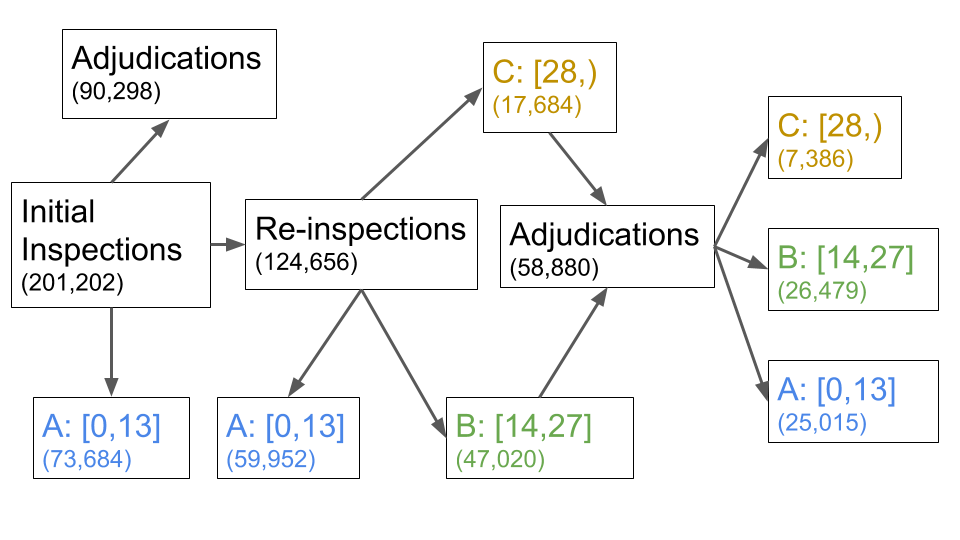
\includegraphics[scale = 0.5]{Figures/Scores.png}
\caption{The Breakdown of Inspections Across the Inspection Cycle.}
\footnotetext{Sample consists of all cycle-inspections after 10/1/2010. The ranges bound by brackets and parentheses represent the score ranges that correspond to the grades.}
\label{pipeline}
\end{figure}

\begin{table}
\centering
\caption{Summary Statistics of Restaurants and Inspections}
\label{sum_stat}
{
\def\sym#1{\ifmmode^{#1}\else\(^{#1}\)\fi}
\begin{tabular}{l*{2}{c}}
\hline\hline
                    &\multicolumn{1}{c}{Restaurant Sample}&\multicolumn{1}{c}{Inspection Sample}\\
                    &        mean&        mean\\
\hline
chain               &       0.112&       0.104\\
Fast Food           &       0.019&       0.016\\
Bar                 &       0.057&       0.061\\
Buffet Service      &       0.015&       0.018\\
Cater Service       &       0.005&       0.004\\
Counter Service     &       0.335&       0.387\\
Take-out Service    &       0.440&       0.386\\
Wait Service        &       0.182&       0.222\\
Cafeteria Service   &       0.010&       0.009\\
\hline\hline
\end{tabular}
}

\footnotetext{This table presents the summary statistics on the sample of inspections after October 1 2010. The restaurant sample contains one observation per restaurant and the inspection sample contains one observation per inspection.}
\end{table}

\newpage 

\begin{figure}[h!]
\centering
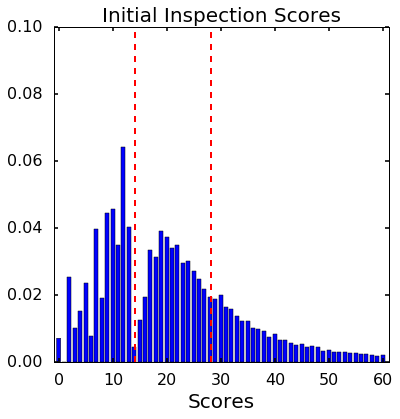
\includegraphics[scale = 0.55]{Figures/init_score.png}
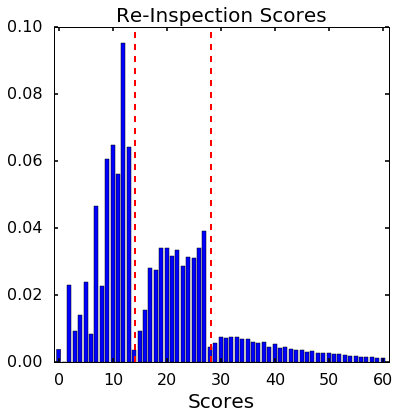
\includegraphics[scale = 0.55]{Figures/re_score.png}
\caption{Score Distribution of Initial Inspections and Re-inspections.}
\label{bunching}
\footnotetext{This figure displays the distribution of inspection scores during initial inspections and re-inspections. The dotted red line represents the 13-14 points and 27-28 thresholds.}
\end{figure}

%%%%%%%%%%%%%%%%%%%%%%%% Inspector Section %%%%%%%%%%%%%%%%%%%%%%%

\begin{figure}[h!]
\centering
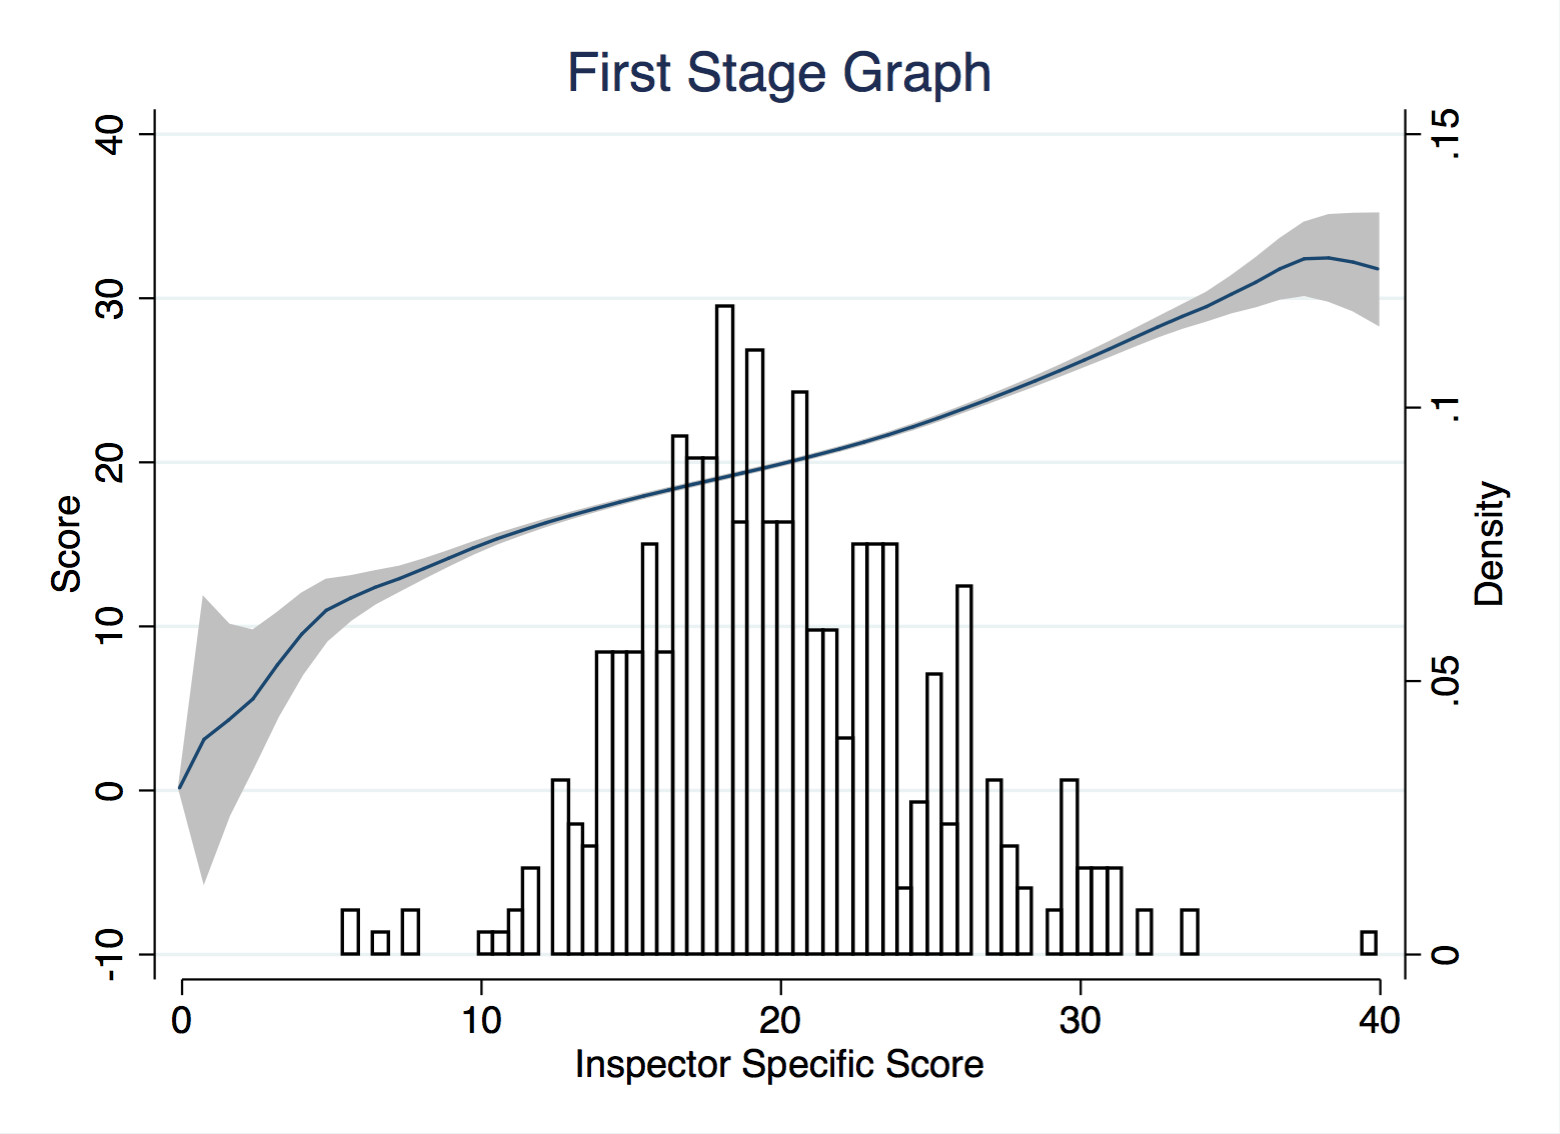
\includegraphics[scale = 0.65]{Figures/first_stage_score.png}
\caption{The plot is generated based on 156,323 initial inspections conducted by inspectors who had done at least 50 initial inspections. The expected inspection score on the left y-axis is plotted against the leave-out average inspector scores on the x-axis. The right axis shows the density of inspector average scores.}
\label{first_stage_fig}
\end{figure}

\newpage

\begin{table}[h!]
\centering
\subfloat[Full]{\begin{tabular}{lccc} \hline
 & (1) & (2) & (3) \\
VARIABLES & Score & Score & Score \\ \hline
 &  &  &  \\
Z & 0.961*** & 0.997*** & 1.135*** \\
 & (0.00948) & (0.00983) & (0.0162) \\
 &  &  &  \\
Observations & 330,469 & 330,466 & 325,681 \\
R-squared & 0.149 & 0.201 & 0.414 \\
Restaurant Controls & NO & YES & NO \\
Restaurant FE & NO & NO & YES \\
 F Statistics & 10271 & 10270 & 4908 \\ \hline
\multicolumn{4}{c}{ Robust standard errors in parentheses} \\
\multicolumn{4}{c}{ *** p$<$0.01, ** p$<$0.05, * p$<$0.1} \\
\end{tabular}
}

\subfloat[Initial Inspections]{\begin{tabular}{lccc} \hline
 & (1) & (2) & (3) \\
VARIABLES & Score & Score & Score \\ \hline
 &  &  &  \\
Z & 0.945*** & 0.952*** & 0.989*** \\
 & (0.0125) & (0.0131) & (0.0147) \\
 &  &  &  \\
Observations & 200,623 & 200,620 & 192,356 \\
R-squared & 0.141 & 0.208 & 0.475 \\
Restaurant Controls & NO & YES & NO \\
Restaurant FE & NO & NO & YES \\
 F Statistics & 5685 & 5264 & 4537 \\ \hline
\multicolumn{4}{c}{ Robust standard errors in parentheses} \\
\multicolumn{4}{c}{ *** p$<$0.01, ** p$<$0.05, * p$<$0.1} \\
\end{tabular}
}

\subfloat[Re-inspections]{\begin{tabular}{lccc} \hline
 & (1) & (2) & (3) \\
VARIABLES & Score & Score & Score \\ \hline
 &  &  &  \\
Z & 0.948*** & 0.959*** & 0.997*** \\
 & (0.0111) & (0.0111) & (0.0150) \\
 &  &  &  \\
Observations & 123,226 & 123,220 & 113,385 \\
R-squared & 0.125 & 0.162 & 0.460 \\
Restaurant Controls & NO & YES & NO \\
Restaurant FE & NO & NO & YES \\
 F Statistics & 7320 & 7528 & 4431 \\ \hline
\multicolumn{4}{c}{ Robust standard errors in parentheses} \\
\multicolumn{4}{c}{ *** p$<$0.01, ** p$<$0.05, * p$<$0.1} \\
\end{tabular}
}
\footnotetext{First column consists of all inspections after 10/1/2010. The sample for the second column is reduced to inspections with non-empty zipcode, chain indicator, cuisine type, venue type, and service type. Standard errors are two-way clustered at the inspector and zipcode level.}
\caption{First Stage Regression of Inspection Score on Inspector Stringency}
\label{first_stage_reg}
\end{table}

\begin{figure}[h!]
\centering
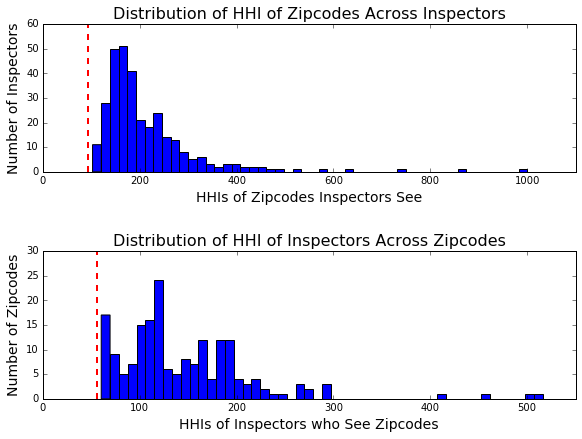
\includegraphics[scale = 0.7]{Figures/zip_herf.png}
\caption{Distribution of HHI}
\label{zip_herf}
\end{figure}

\begin{table}[h!]
\scalebox{0.65}{
\begin{tabular}{lcccccc} \hline
VARIABLES & Score &  & Inspector Stringency &     & Inspector Stringency  &  \\ 
VARIABLES & (> 50 Inspections) & se &  (> 50 Inspections) & se & (> 650 Inspections) & se \\ \hline
last score & 0.218*** & (0.00746) & -0.000440 & (0.00199) & -0.00193 & (0.00205) \\
last grade = B & 1.430*** & (0.131) & 0.0178 & (0.0628) & 0.0837 & (0.0683) \\
last grade = C & 1.495*** & (0.206) & -0.0494 & (0.0764) & 0.0240 & (0.0807) \\
last inspector propensity & -0.298*** & (0.0104) & -0.00363 & (0.00491) & -0.00529 & (0.00551) \\
chain & -3.644*** & (0.179) & -0.0274 & (0.0644) & -0.0300 & (0.0734) \\
Sea Food & 0.301 & (0.412) & -0.0687 & (0.129) & -0.0648 & (0.136) \\
Chinese & 1.588*** & (0.307) & -0.0952* & (0.0510) & -0.0511 & (0.0546) \\
Pizza/Italian & 0.305** & (0.118) & -0.0893*** & (0.0342) & -0.0614 & (0.0384) \\
Coffee/Tea & -2.219*** & (0.162) & -0.0421 & (0.0889) & -0.0514 & (0.0966) \\
Latin & 1.534*** & (0.303) & -0.0714 & (0.0556) & -0.0390 & (0.0583) \\
Spanish & 1.560*** & (0.261) & 0.0125 & (0.0615) & -0.0435 & (0.0691) \\
Caribbean & 1.542*** & (0.288) & -0.0637 & (0.0608) & -0.0619 & (0.0544) \\
Sandwich & 0.661** & (0.297) & -0.00916 & (0.0472) & 0.0180 & (0.0488) \\
Concession Stands & -4.379*** & (0.722) & 0.295 & (0.197) & 0.209 & (0.211) \\
Fast Food Restaurant-Food Court & 0.570*** & (0.187) & 0.0394 & (0.0881) & -0.0211 & (0.0868) \\
Restaurant  & 1.453*** & (0.158) & 0.0449 & (0.0662) & 0.00343 & (0.0641) \\
Buffet Service & 2.564*** & (0.365) & -0.182* & (0.107) & -0.196 & (0.118) \\
Cater Service & -1.897*** & (0.609) & -0.200 & (0.190) & -0.193 & (0.219) \\
Counter Service & -0.635*** & (0.185) & 0.0273 & (0.0613) & 0.0123 & (0.0684) \\
Take-out Service & -1.410*** & (0.185) & -0.153 & (0.110) & -0.173 & (0.123) \\
Wait Service & 1.205*** & (0.166) & 0.0418 & (0.0481) & 0.0404 & (0.0525) \\
Cafeteria Service & -3.541*** & (0.500) & -0.280* & (0.156) & -0.200 & (0.168) \\
Observations & 299,174 &  & 299,174 &  & 244,099 &  \\
 F Statistics & 101.6 &  & 2.423 &  & 2.249 &  \\ \hline
\multicolumn{7}{c}{ Robust standard errors in parentheses} \\
\multicolumn{7}{c}{ *** p$<$0.01, ** p$<$0.05, * p$<$0.1} \\
\end{tabular}
}
\footnotetext{Table shows the result of regressing Inspector Leniency on Restaurant characteristics and previous inspection results. Most variables that are highly predictive of restaurant scores are not predictive of inspector propensity, with the exception of the indicator for whether the establishment is a bar or offers wait service. The regressions include date, zipcode, inspection type fixed effects, and the errors are two-way clustered at the inspector and restaurant level.}
\caption{}
\label{cond_ind}
\end{table}

\begin{table}
\subfloat[Full Sample]{
\begin{tabular}{lcccc} \hline
 & (1) & (2) & (3) & (4) \\
VARIABLES & OLS & OLS & IV & IV \\ \hline
 &  &  &  &  \\
Score & 0.182*** & 0.134*** & -0.262*** & -0.233*** \\
 & (0.00763) & (0.00654) & (0.0330) & (0.0253) \\
 &  &  &  &  \\
Observations & 156,323 & 156,317 & 156,323 & 156,317 \\
Restaurant Controls & No & Yes & No & Yes \\
 Restaurant FE & No & No & No & No \\ \hline
\multicolumn{5}{c}{ Robust standard errors in parentheses} \\
\multicolumn{5}{c}{ *** p$<$0.01, ** p$<$0.05, * p$<$0.1} \\
\end{tabular}
}

\subfloat[Score > 13]{
\begin{tabular}{lcccc} \hline
 & (1) & (2) & (3) & (4) \\
VARIABLES & OLS & OLS & IV & IV \\ \hline
 &  &  &  &  \\
Score & 0.155*** & 0.129*** & -0.283*** & -0.252*** \\
 & (0.00726) & (0.00680) & (0.0363) & (0.0314) \\
next score & 0.145*** & 0.112*** & -0.130*** & -0.126*** \\
 & (0.00617) & (0.00564) & (0.0119) & (0.0114) \\
 &  &  &  &  \\
Observations & 101,385 & 101,377 & 101,382 & 101,374 \\
Restaurant Controls & No & Yes & No & Yes \\
 Restaurant FE & No & No & No & No \\ \hline
\multicolumn{5}{c}{ Robust standard errors in parentheses} \\
\multicolumn{5}{c}{ *** p$<$0.01, ** p$<$0.05, * p$<$0.1} \\
\end{tabular}
}

\subfloat[Score $\leq$ 13]{
\begin{tabular}{lcccc} \hline
 & (1) & (2) & (3) & (4) \\
VARIABLES & OLS & OLS & IV & IV \\ \hline
 &  &  &  &  \\
Score & 0.613*** & 0.398*** & -3.041*** & -1.902*** \\
 & (0.0229) & (0.0209) & (0.532) & (0.256) \\
 &  &  &  &  \\
Observations & 51,451 & 51,442 & 51,451 & 51,442 \\
Restaurant Controls & No & Yes & No & Yes \\
 Restaurant FE & No & No & No & No \\ \hline
\multicolumn{5}{c}{ Robust standard errors in parentheses} \\
\multicolumn{5}{c}{ *** p$<$0.01, ** p$<$0.05, * p$<$0.1} \\
\end{tabular}
}
\caption{Impact of Inspection Score on Subsequent Inspection Result}
\footnotetext{Standard errors are two-way clustered at zipcode and inspector levels.}
\label{score_impact}
\end{table}

\begin{table}
\centering
\scalebox{0.9}{\begin{tabular}{lcccccc} \hline
 & (1) & (2) & (3) & (4) & (5) & (6) \\
VARIABLES & Score (OLS) & Score (IV) & Closure (OLS) & Closure (IV) & Grade A (OLS) & Grade A (IV) \\ \hline
 &  &  &  &  &  &  \\
Score & -0.139*** & -0.242*** & -0.000763*** & -0.00101*** & -8.49e-05 & 0.00222*** \\
 & (0.00492) & (0.0162) & (8.26e-05) & (0.000185) & (0.000127) & (0.000556) \\
 &  &  &  &  &  &  \\
Observations & 149,831 & 149,831 & 138,674 & 138,674 & 149,831 & 149,831 \\
Inspection Date FE & YES & YES & YES & YES & YES & YES \\
Restaurant FE & YES & YES & YES & YES & YES & YES \\
 dependent mean & 21.08 & 21.08 & 0.0162 & 0.0162 & 0.372 & 0.372 \\ \hline
\multicolumn{7}{c}{ Robust standard errors in parentheses} \\
\multicolumn{7}{c}{ *** p$<$0.01, ** p$<$0.05, * p$<$0.1} \\
\end{tabular}
}
\caption{Impact of Inspection Scores on Temporary Closure and Obtaining Grade A}
\label{Shutdown_A}
\footnotetext{Standard errors are two-way clustered at zipcode and inspector levels.}
\end{table}

\begin{figure}
\centering
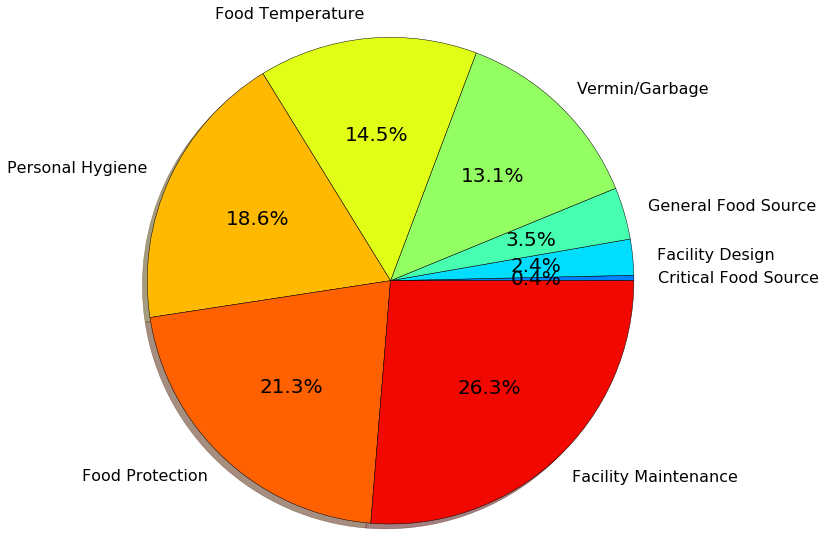
\includegraphics[scale = 0.5]{Figures/viol_group_pie.png}
\caption{Breakdown of Frequencies of Violation Groups}
\label{task_pie}
\end{figure}

\begin{sidewaystable}[]
\scalebox{0.75}{
\begin{tabular}{lcccccccc} \hline
 & (1) & (2) & (3) & (4) & (5) & (6) & (7) & (8) \\
VARIABLES & Facility Maintenance & Food Protection & Personal Hygiene & Food Temperature & Vermin/Garbage & Gen. Food Source & Facility Design & Crit. Food Source \\ \hline
 &  &  &  &  &  &  &  &  \\
Facility Maintenance & \cfbox{red}{1.012***} & -0.0212 & 0.0411*** & 0.00688 & 0.00619 & 0.000455 & -0.0111 & 0.00262 \\
 & (0.0193) & (0.0202) & (0.0143) & (0.0151) & (0.0213) & (0.0117) & (0.0103) & (0.00166) \\
Food Protection & -0.0597 & \cfbox{red}{0.940***} & 0.0543 & 0.234*** & 0.0642 & 0.0196 & -0.0107 & 0.00770 \\
 & (0.0637) & (0.0557) & (0.0494) & (0.0600) & (0.0629) & (0.0386) & (0.0295) & (0.00536) \\
Personal Hygiene & 0.0581*** & 0.0394** & \cfbox{red}{0.965***} & 0.0898*** & 0.0651*** & 0.0439*** & 0.0326*** & 0.00183 \\
 & (0.0170) & (0.0187) & (0.0146) & (0.0198) & (0.0195) & (0.0133) & (0.00927) & (0.00211) \\
Food Temperature & 0.0310 & 0.113*** & 0.0177 & \cfbox{red}{0.906***} & 0.0999*** & 0.0369*** & 0.0442*** & 0.00192 \\
 & (0.0202) & (0.0240) & (0.0167) & (0.0222) & (0.0246) & (0.0134) & (0.00993) & (0.00156) \\
Vermin/Garbage & 0.0449 & 0.0280 & -0.0909** & \cfbox{blue}{-0.178***} & \cfbox{red}{0.908***} & -0.0261 & 0.0158 & -0.00511 \\
 & (0.0540) & (0.0465) & (0.0442) & (0.0564) & (0.0520) & (0.0346) & (0.0253) & (0.00504) \\
Gen. Food Source & -0.0560* & -0.0629* & 0.00496 & -0.0256 & -0.0760** & \cfbox{red}{0.947***} & -0.0262 & -0.000915 \\
 & (0.0317) & (0.0353) & (0.0286) & (0.0281) & (0.0350) & (0.0241) & (0.0159) & (0.00359) \\
Facility Design & -0.184*** & \cfbox{blue}{-0.337***} & 0.0223 & 0.00730 & \cfbox{blue}{-0.400***} & \cfbox{blue}{-0.168***} & \cfbox{red}{0.791***} & -0.00582 \\
 & (0.0631) & (0.0824) & (0.0515) & (0.0731) & (0.0739) & (0.0408) & (0.0457) & (0.00844) \\
Crit. Food Source & -0.130 & -0.132 & -0.199 & -0.111 & 0.0138 & -0.265 & -0.0209 & \cfbox{red}{0.891***} \\
 & (0.204) & (0.237) & (0.151) & (0.213) & (0.229) & (0.173) & (0.114) & (0.0334) \\
 &  &  &  &  &  &  &  &  \\
Observations & 337,615 & 337,615 & 337,615 & 337,615 & 337,615 & 337,615 & 337,615 & 337,615 \\
 Time FE & YES & YES & YES & YES & YES & YES & YES & YES \\ \hline
\multicolumn{9}{c}{ Robust standard errors in parentheses} \\
\multicolumn{9}{c}{ *** p$<$0.01, ** p$<$0.05, * p$<$0.1} \\
\end{tabular}}
\footnotetext{Standard errors are two-way clustered at zipcode and inspector levels}
\caption{}
\label{multi_first_reg}
\end{sidewaystable}

\begin{sidewaystable}[h!]
\centering
\scalebox{0.75}{
\begin{tabular}{lcccccccc} \hline
 & (1) & (2) & (3) & (4) & (5) & (6) & (7) & (8) \\
VARIABLES & Facility Maintenance & Food Protection & Personal Hygiene & Food Temperature & Vermin/Garbage & Gen. Food Source & Facility Design & Crit. Food Source \\ \hline
 &  &  &  &  &  &  &  &  \\
Facility Maintenance & \textcolor{red}{-0.236***} & 0.00733 & 0.000184 & -0.00506 & -0.000922 & -0.00159 & 0.000981 & -0.000509 \\
 & (0.00961) & (0.0119) & (0.0107) & (0.00944) & (0.00766) & (0.00380) & (0.00295) & (0.00140) \\
Food Protection & \textcolor{blue}{-0.0776**} & \textcolor{red}{-0.177***} & -0.00731 & -0.0142 & \textcolor{blue}{-0.0397*} & -0.0100 & 0.00372 & \textcolor{brown}{0.00780*} \\
 & (0.0378) & (0.0306) & (0.0410) & (0.0253) & (0.0227) & (0.0113) & (0.0108) & (0.00400) \\
Personal Hygiene & 0.0222 & -0.00484 & \textcolor{red}{-0.189***} & -0.00771 & -0.000551 & 0.00458 & 0.00129 & 0.00217 \\
 & (0.0156) & (0.0103) & (0.0148) & (0.00957) & (0.00892) & (0.00489) & (0.00320) & (0.00173) \\
Food Temperature & 0.0148 & -0.0261 & 0.0133 & \textcolor{red}{-0.214***} & -0.00923 & 0.00613 & -0.00622 & -0.00153 \\
 & (0.0216) & (0.0163) & (0.0162) & (0.0134) & (0.0128) & (0.00722) & (0.00573) & (0.00243) \\
Vermin/Garbage & \textcolor{brown}{0.132***} & \textcolor{blue}{-0.0784*} & 0.00134 & 0.0446 & \textcolor{red}{-0.174***} & 0.0128 & -0.0105 & -0.00126 \\
 & (0.0439) & (0.0404) & (0.0544) & (0.0318) & (0.0283) & (0.0159) & (0.0138) & (0.00404) \\
Gen. Food Source & -0.0114 & -0.00139 & -0.0456 & -0.0103 & \textcolor{blue}{-0.0395*} & \textcolor{red}{-0.191***} & -0.0147 & -0.000895 \\
 & (0.0291) & (0.0348) & (0.0374) & (0.0334) & (0.0202) & (0.0199) & (0.00933) & (0.00395) \\
Facility Design & 0.0265 & \textcolor{blue}{-0.195**} & -0.00742 & 0.0168 & -0.0235 & 0.00421 & \textcolor{red}{-0.199***} & \textcolor{brown}{0.0169*} \\
 & (0.0787) & (0.0925) & (0.0776) & (0.0551) & (0.0612) & (0.0296) & (0.0239) & (0.00977) \\
Crit. Food Source & 0.274 & -0.284 & 0.279 & 0.125 & -0.0346 & -0.0233 & -0.0643 & \textcolor{red}{-0.185***} \\
 & (0.248) & (0.207) & (0.244) & (0.195) & (0.142) & (0.0848) & (0.0682) & (0.0298) \\
Observations & 149,831 & 149,829 & 149,831 & 149,829 & 149,829 & 149,831 & 149,829 & 149,831 \\
Dependent mean & 0.989 & 0.802 & 0.842 & 0.645 & 0.503 & 0.125 & 0.0694 & 0.0126 \\ \hline
\multicolumn{9}{c}{ Robust standard errors in parentheses} \\
\multicolumn{9}{c}{ *** p$<$0.01, ** p$<$0.05, * p$<$0.1} \\
\end{tabular}
}
\caption{}
\footnotetext{Standard errors are two-way clustered at zipcode and inspector levels.}
\end{sidewaystable}

\begin{sidewaystable}[]
    \centering
    \scalebox{0.75}{
\begin{tabular}{lcccccccc} \hline
 & (1) & (2) & (3) & (4) & (5) & (6) & (7) & (8) \\
VARIABLES & Facility Maintenance & Food Protection & Personal Hygiene & Food Temperature & Vermin/Garbage & Gen. Food Source & Facility Design & Crit. Food Source \\ \hline
 &  &  &  &  &  &  &  &  \\
Facility Maintenance & \cfbox{red}{-0.0299**} & -0.0304** & -0.0131 & -0.0372** & -0.0437** & -0.00911 & -0.00103 & 0.00330 \\
 & (0.0134) & (0.0142) & (0.0148) & (0.0148) & (0.0184) & (0.00866) & (0.00569) & (0.00264) \\
Food Protection & 0.0134 & \cfbox{red}{-0.106**} & -0.0282 & -0.251*** & -0.155*** & -0.0612*** & 0.000699 & 0.0166* \\
 & (0.0398) & (0.0487) & (0.0466) & (0.0456) & (0.0567) & (0.0231) & (0.0259) & (0.00853) \\
Personal Hygiene & 0.0136 & -0.0767*** & \cfbox{red}{-0.0583***} & -0.106*** & -0.0804*** & -0.0219** & -0.00694 & 0.00373 \\
 & (0.0160) & (0.0177) & (0.0190) & (0.0185) & (0.0210) & (0.00967) & (0.00697) & (0.00372) \\
Food Temperature & -0.0215 & -0.122*** & -0.0202 & \cfbox{red}{-0.0869***} & -0.108*** & -0.00905 & -0.0246*** & -0.00258 \\
 & (0.0185) & (0.0198) & (0.0163) & (0.0200) & (0.0222) & (0.0131) & (0.00894) & (0.00437) \\
Vermin/Garbage & -0.00984 & -0.0749** & -0.0152 & 0.0950*** & \cfbox{red}{-0.0675*} & 0.0262 & -0.0221 & -0.00139 \\
 & (0.0292) & (0.0307) & (0.0367) & (0.0337) & (0.0388) & (0.0168) & (0.0203) & (0.00550) \\
Gen. Food Source & -0.0120 & -0.0154 & -0.0410* & -0.0359 & -0.0459* & \cfbox{red}{-0.0227} & -0.0222** & 0.000948 \\
 & (0.0173) & (0.0236) & (0.0214) & (0.0235) & (0.0262) & (0.0147) & (0.00881) & (0.00399) \\
Facility Design & -0.0241 & -0.137*** & -0.0732 & -0.0378 & -0.152*** & 0.0154 & \cfbox{red}{-0.0247} & 0.0205** \\
 & (0.0365) & (0.0473) & (0.0505) & (0.0452) & (0.0526) & (0.0248) & (0.0236) & (0.00838) \\
Crit. Food Source & -0.0391 & -0.258** & 0.102 & -0.114 & -0.0939 & 0.00645 & 0.00234 & \cfbox{red}{-0.0492*} \\
 & (0.136) & (0.131) & (0.125) & (0.150) & (0.136) & (0.0698) & (0.0703) & (0.0258) \\
 &  &  &  &  &  &  &  &  \\
 Observations & 156,317 & 156,316 & 156,316 & 156,317 & 156,317 & 156,316 & 156,316 & 156,316 \\ \hline
\multicolumn{9}{c}{ Robust standard errors in parentheses} \\
\multicolumn{9}{c}{ *** p$<$0.01, ** p$<$0.05, * p$<$0.1} \\
\end{tabular}   
}
\caption{}
\label{multi_second_reg}
\footnotetext{Standard errors are two-way clustered at zipcode and inspector levels}
\end{sidewaystable}

\begin{table}
\scalebox{0.9}{
\begin{tabular}{lcccc} \hline
 & (1) & (2) & (3) & (4) \\
VARIABLES & Initial Inspections & Re-inspections (OLS) & Re-inspections (OLS) & Re-inspections (IV) \\ \hline
 &  &  &  &  \\
Score & 0.000219 & 0.00143*** &  & 0.00160*** \\
 & (0.000208) & (0.000236) &  & (0.000532) \\
Days Until Next & 0.000380*** & 0.000434*** & 0.000125*** & 0.000182*** \\
 & (3.78e-05) & (4.76e-05) & (2.04e-05) & (3.86e-05) \\
Modified Score &  &  & 0.00222*** &  \\
 &  &  & (0.000250) &  \\
 &  &  &  &  \\
 Observations & 136,276 & 83,361 & 83,361 & 83,361 \\ \hline
\multicolumn{5}{c}{ Robust standard errors in parentheses} \\
\multicolumn{5}{c}{ *** p$<$0.01, ** p$<$0.05, * p$<$0.1} \\
\end{tabular}}
\caption{}
\footnotetext{Sample include inspections conducted by inspectors who have conducted at least 50 inspections of the same type. Standard errors are two-way clustered at zipcode and inspector levels.}
\label{complaint_table}
\end{table}

\subsection{Matching 311 calls to Food Inspection Data}
I use fuzzystring matching to link 311 complaint calls with food inspection data based on the address. I perform steps to standardize the address
\begin{itemize}
\item Add suffix to numbered streets, i.e. change "1 Street" to "1st Street"
\end{itemize}
[TODO: to be completed]

\end{document}

%%%%%%%%%%%%%%%%%%%%%%%%%%%%%%%%%%%%%%%%%%%%%%%%%%%%%%%%%%%%%%%%%%%%%%%%%%%%%%%%%%%%%%%%%%%%%%%%%%%%%%%%%%%%%%%%%%%%%%%%%%%%%%%%%%%%%%%%%%%%%%%%%%%%%%%%%%%%%%%%%%%%%%%%%%%%%%%%

\begin{table}[h!]
\centering
\begin{tabular}{lccc} \hline
 & (1) & (2) & (3) \\
VARIABLES & Initial Inspections & Re-inspections (OLS) & Re-inspections (IV) \\ \hline
 &  &  &  \\
not\_A & 0.00240 & 0.0602*** & 0.108*** \\
 & (0.00814) & (0.00453) & (0.0110) \\
Days Until Next & 0.000395*** & 0.000158*** & 0.000227*** \\
 & (4.38e-05) & (1.97e-05) & (2.59e-05) \\
 &  &  &  \\
 Observations & 136,389 & 85,626 & 85,626 \\ \hline
\multicolumn{4}{c}{ Robust standard errors in parentheses} \\
\multicolumn{4}{c}{ *** p$<$0.01, ** p$<$0.05, * p$<$0.1} \\
\end{tabular}
\caption{Impact of Not Getting an A on Frequencies of Complaint Calls}
\label{not_A_table}
\footnotetext{Standard errors two-way clustered at zipcode and inspector levels.}
\end{table}


To do so, I turn again to the use of inspector assignments to instrument for the letter grade. Given that I have one instrument, I create a new variable called $not\_A$, which is a dummy variable that equals 1 if modified score is above 13. I estimate the following equation.\footnote{Regressing with modified score as the endogenous variable may lead to the violation of the monotonicity condition. To see this, suppose a restaurant gets a lenient inspector and earns 12. The restaurant earns an A, faces no fine, and does not pursue adjudication. Hence its modified score is also 12. But suppose that had the restaurant gotten a stringent inspector, it would have gotten a 14, which causes the establishment to pursue adjudication that results in a modified lower than 12.} 
\begin{align*}
Complaints_{it} = \beta not\_A_{it} + \theta Days\_to\_next_{it} + \delta_i + \tau_t + \varepsilon. 
\end{align*}
In the case of re-inspection, $Complaints_{it}$ and $Days\_to\_next$ are calculated as the total number of complaints and number of days between the either adjudication date and inspection date, whichever is later, to the next initial inspection date, respectively. Table \ref{not_A_table} reports the result. We again see that inspection result from the initial inspection has very little effect on the frequencies of calls. On the other hand, not getting an A during the re-inspection is associated with a significant increase in complaint calls. The IV regression is estimating the LATE on restaurants that got scores above 13 and were not able to get the score modified to be below 13 during adjudication. 

\begin{subequations}
\begin{align}
Complaints_{it} = \sum_{i} \beta_i \textbf{1}_{\{Score_{it} = i\}} + \theta Days\_to\_next_{it} + \delta_i + \tau_t + \varepsilon,  \label{non_param_score} \\
Complaints_{it} = \sum_{i} \beta_i \textbf{1}_{\{Modified Score_{it} = i\}} + \theta Days\_to\_next_{it} + \delta_i + \tau_t + \varepsilon. \label{non_param_modscore}
\end{align}
\end{subequations}
Modified scores, rather than scores, determine the letter grades. I calculate $Days\_to\_next_{it}$ for the modified score regression as the days between adjudication date and the next initial inspection date. If lower letter grades causes customers to call in more frequently, then we expect the $\beta_i$ estimates to jump between $\beta_{13}$ and $\beta_{14}$ and between $\beta_{27}$ and $\beta_{28}$ for \eqref{non_param_modscore} but not \eqref{non_param_score}. 


\begin{figure}[h!]
\centering
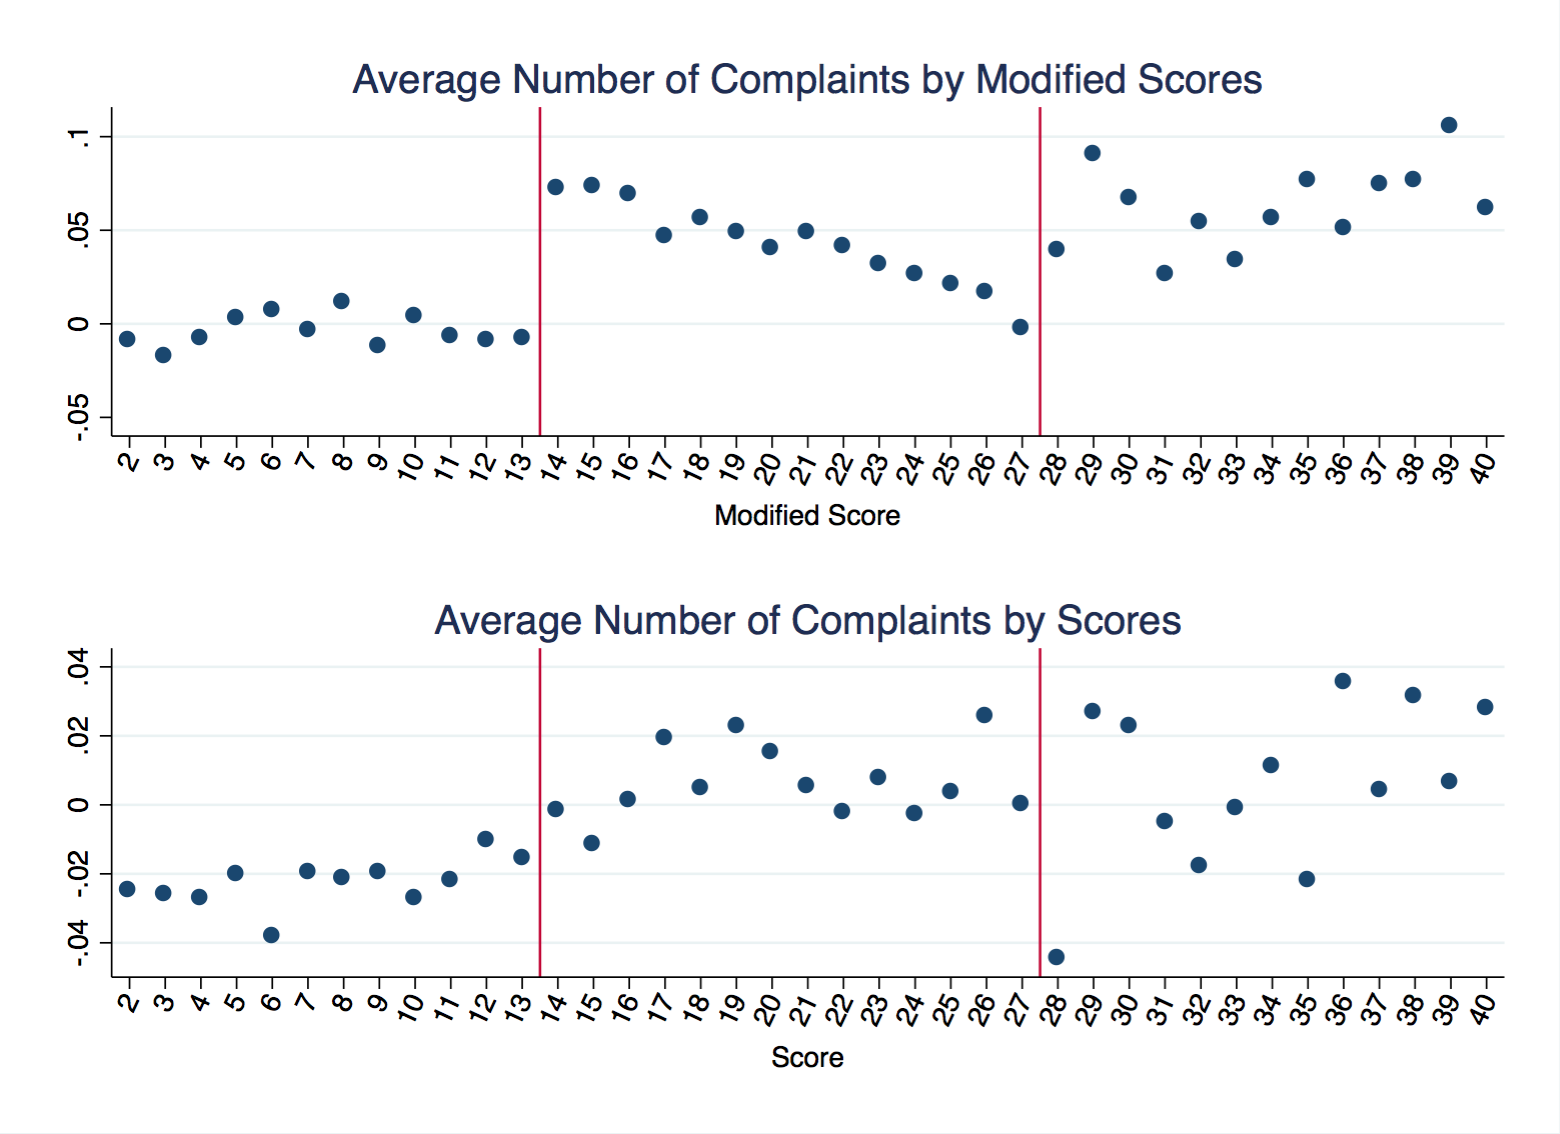
\includegraphics[scale = 0.6]{non_param.png}
\caption{}
\footnotetext{Sample includes re-inspections conducted by inspectors who have done at least 50 re-inspections. Observations with more than 4 complaints are excluded.}
\label{non_param_fig}
\end{figure}

However, little empirical evidence exists that examines the efficacies of these inspections. The first difficulty is the data availability. Analysis requires access to administrative level data from various government agencies. These data sources have become easier to access, thanks to advances in data management of large datasets and the Freedom of Information Act that require government agencies to make certain records publically available. The second 

I also consider the effect of the modified scores on subsequent inspection scores. 
\begin{align}
        Score_{i,t^{next}} = \beta Mod\_Score_{i,t} + \delta_i + \tau_{t} + \tau_{t^{next}} + \varepsilon_{it},
        \label{mod}
\end{align}
where the equation \eqref{mod} is the same as \eqref{score} with $SCORE_{it}$ switched with $Mod\_Score_{it}$. We may expect the result to be different the modified scores, rather than the original inspection scores, determine the fines issued. We restrict the regression to initial inspections with scores higher than 13.\footnote{Including initial inspections with scores lower than 13 may violate the monotonicity condition. To see this, suppose a restaurant gets a lenient inspector and earns 12. The restaurant earns an A, faces no fine, and does not pursue adjudication. Hence its modified score is also 12. But suppose that had the restaurant gotten a stringent inspector, it would have gotten a 14, which causes the establishment to pursue adjudication that results in a modified lower than 12.}


\subsection{Impact of Inspection Results on Restaurant Closure}

The food inspection data do not have information on the exact date of closure. Since 99\% of inspections are at most 530 days apart, I encode 

Since the subsequent inspections following inspections with higher scores occur earlier, pooling all the inspections biases the result. Surviving restaurants that received higher scores appear more often in the data than those that gotten lower scores, 

To address this issue, I create a restaurant-year level panel data. I estimate the following equation
\begin{align*}
Pr(Open_{it}) = \delta_i + \tau_t + \beta Score^{avg}_{it} + \varepsilon_{it}
\end{align*}
where $\delta_i$ and $\tau_t$ is restaurant and year fixed effect, $Open_{it}$ is an indicator variable that equals 1 if there is at least one inspection after year $t$, 

By studying the impact of food inspections on restaurant survival, this paper also contributes to the literature of regulatory costs on the businesses. \cite{kleiner_00} finds that occupational licensing policies in the field of dentistry do not improve quality of service but increases prices. \cite{greenstone_12} find that stricter air pollution regulation decreases total factor productivity of surviving plants. In France where firms with 50 or more workers face substantially more regulations, \cite{Gourio_Roys_14} find that abnormally many firms have only 49 works, citing this bunching as evidence for the regulations' distortionary effect.

Two critical components of my empirical strategy are the random assignment of food inspectors and the different levels of leniency across inspectors. These two factors allow me to use inspector fixed effects as an instrumental variable for each inspection result.\footnote{Other papers that use the random assignments of judges, inspectors, or reviewers to estimate the causal impact of government policies include \cite{Doyle_07, Doyle_08} and \cite{Maestas_13}.} To better illustrate this point, consider the thought experiment of two identical restaurants, with one randomly assigned a strict inspector and who assigns a poor grade and the other assigned a lenient inspector who assigns a good grade. Because of the randomness of the inspector assignments, we can use the difference in the observed outcomes between the two restaurants as the causal impact of the inspection results. Finally, since the inspections are conducted once a year, the food inspection data also tracks the survival rate of restaurants across time. Combining this with the empirical strategy I described above also allows me to answer whether this policy has hurt local businesses. 



The main resource from IRISS that I'd like to access is Sherlock GPU. My data set contain over 500,000 inspections, and for each inspection, I have up to 80 different types of violations. For certain regression, specification, I may have over 10's of millions of observation, and being able to use the GPU will allow faster computation that allows me to experiment with more empirical specifications. 

I supplement the literature by my choice of outcome variables and my methodology. While I also use results from food inspections as measures for restaurant cleanliness, I exploit the randomness of inspector assignments to estimate the causal impact of third-party monitoring on subsequent compliance behaviors

My study also fits in with a broader principal-agent literature that examines the interaction between government regulations and compliance behaviors. For example, \cite{Duflo_Greenstone_14} study how increased frequencies of environmental inspections influence pollution from plants. \cite{Gemmell_Ratto_12} and \cite{Kleven_Waseem_13} measure the impact of tax audits on tax non-compliance behaviors.

These policies for better transparency have the potentials to improve social welfare through two channels: demand side and supply side. For the demand side, these grades inform the customers so that they can avoid restaurants with poor food sanitation qualities. There is strong evidence that consumers respond to these posted grades\footnote{\cite{jie_leslie_05} and \cite{jie_leslie_09} combine inspection grades with tax revenue data and find evidence that consumer choices responds to the posted grades. Restaurants that enjoy upgrades see increases in revenues while places that suffer downgrades experience drops in revenues.}. For the supply side, having to post their food inspection results may incentivize restaurants to improve their overall cleanliness. However, the evidence on the supply side is more mixed\footnote{\cite{jie_leslie_05} and \cite{Simon_05} find strong evidence for decrease in hospitalization for foodborne illnesses in jurisdictions in Los Angeles following the enactments of the grading systems. On the other hand, by using 311 complaint calls and Google Trend of search terms related to food poisoning as measures for sanitation conditions, \cite{Ho_2012} finds no evidence that rates of foodborne illnesses changed New York City instituted its grading system.}\footnote{A major shortcoming of using the number of foodborne illnesses is that it is a very noisy measure. Food poisoning often goes unreported and cannot easily be traced back to the original establishment. Instead, \cite{Wong_at_el_2015} and \cite{Meltzer_2015} use inspection scores to measure restaurant cleanliness. After finding that improved sanitation scores and lower violation fines following the reform, they conclude that the reform improved sanitation practices. However, because of the two studies' lack of comparable control groups, they cannot rule out the possibility that changes in other confounding factors such as food sanitation standards following the reform led to the observed changes in the variables of interest. 
}. Opponents of these policies, however, have pointed out that they pose unnecessary compliance costs and hurt local businesses. 
